\documentclass[border=4pt]{standalone}
\usepackage{tikz}
\usetikzlibrary{arrows.meta,calc,shapes.geometric}

\begin{document}
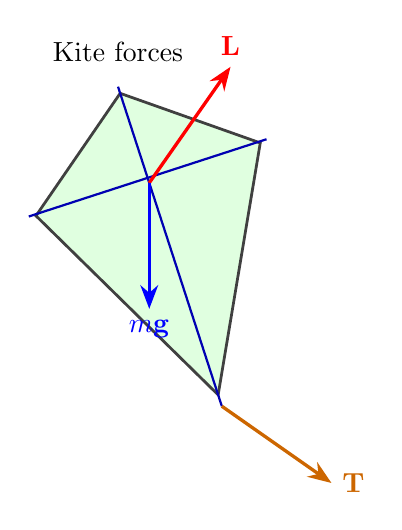
\begin{tikzpicture}[>=Stealth]
  \node[kite,kite vertex angles=105 and 55,shape border uses incircle,
    shape border rotate=18,minimum width=30mm,minimum height=40mm,
    draw=black!75,fill=green!12,line width=1pt,outer sep=2pt] (sail) at (0,0) {};
  \draw[blue!70!black,thick] (sail.upper vertex) -- (sail.lower vertex);
  \draw[blue!70!black,thick] (sail.left vertex) -- (sail.right vertex);
  \draw[-{Stealth[length=3mm]},red,line width=1.2pt]
    (sail.center) -- ++(55:18mm) node[above] {$\mathbf L$};
  \draw[-{Stealth[length=3mm]},blue,line width=1.2pt]
    (sail.center) -- ++(-90:16mm) node[below] {$m\mathbf g$};
  \draw[-{Stealth[length=3mm]},orange!80!black,line width=1.2pt]
    (sail.lower vertex) -- ++(-35:17mm) node[right] {$\mathbf T$};
  \node[above=2mm] at (sail.upper vertex) {Kite forces};
\end{tikzpicture}
\end{document}
